%!TEX TS-program = xelatex
%!TEX encoding = UTF-8 Unicode

\documentclass[12pt]{article}
\usepackage{geometry}                % See geometry.pdf to learn the layout options. There are lots.
\geometry{a4paper}                   % ... or a4paper or a5paper or ... 
%\geometry{landscape}                % Activate for for rotated page geometry
\usepackage[parfill]{parskip}    % Activate to begin paragraphs with an empty line rather than an indent
\usepackage{graphicx}
\usepackage{amssymb}
\usepackage{pstricks,pst-node,pst-text,pst-3d,pst-tree}
\usepackage{hyperref}
\usepackage{float}
\usepackage{wrapfig}
\usepackage{soul}
\usepackage{natbib}


\usepackage{fontspec,xltxtra,xunicode}
\defaultfontfeatures{Mapping=tex-text}
\setromanfont[Mapping=tex-text]{Times New Roman}
\setsansfont[Scale=MatchLowercase,Mapping=tex-text]{Helvetica}
\setmonofont[Scale=MatchLowercase]{Monaco}

\title{Solution to COMP5121 Assignment 2}
\author{QING Pei, 11500811G}
%\date{}                                           % Activate to display a given date or no date

\begin{document}
\maketitle

\setcounter{tocdepth}{2}
\tableofcontents

\section{Problem 1}
\subsection{Negative Association Rule} % (fold)
\label{sub:negative_association_rule}
Association rules are rules like $A\rightarrow B$, which means, in a transaction context, the existence of A in a transaction imply B may also appear in that transaction. $A$ and $B$ may be single items, or they may be itemsets. By ``negative'', we mean one or more items in A and B can be the absence of an item according to Antonie \& Za{\"\i}ane.

This is not the only definition. Savasere's understanding of negative association rules is different. For rule $A\rightarrow B$, it is positive if the real support of $A\cup B$ is significantly higher than the expectation. On contrary, it is negative when the real support is significantly lower than expectation.

Anyway, we search for negative associations to identify products that conflict with each other (so customers buy the one they like and would never touch the one they hate) or complement each other (so the customers buy one and they do not need to another similar product).
% subsection negative_association_rule (end)

\subsection{Interesting Negative Association Rules are Hard to Find} % (fold)
\label{sub:interesting_negative_association_rules_are_hard_to_find}
Compared with the numerous methods proposed to find positive association rules, much fewer have been there for negative association rules. It is difficult to find ``interesting'' negative rules.

In positive rule mining, the data only contains items in the transaction. To mine negative rules, all the items is considered for a transaction, either for its appearance or for its absence. This generates a lot more data to process. Originally the transaction matrix is very sparse, if all those 0s are meaningful and should be considered, the process is far more time-consuming.

Also, it is highly possible that many items do not even occur once in the transactions data. A lot of negative association rules can be generated with such items. But most of them are not interesting. Filtering these kind of rules out as early in the mining algorithm as possible is not a straightforward job.
% subsection interesting_negative_association_rules_are_hard_to_find (end)

\subsection{Find Negative Association Rules} % (fold)
\label{sub:find_negative_association_rules}
The general problem is hard to solve, so further assumptions or information about data are introduced to assist the calculations. In this way, people are able to find a subset of the negative association rules which are interesting.

If we have a complete taxonomy, we may use that info to help mine negative association rules. Assume that items that belong to the same parent in a taxonomy are expected to have similar types of association with other items. That is the \emph{uniformity assumption} by Savasere et al. Together with the taxonomy as \emph{domain knowledge}, we form expectations. The fact may deviate from the expectation. If the deviation from expectation is significant enough, that is call an interesting one. So the mining process is:
\begin{enumerate}
	\item Find the large frequent itemsets
	\item Use domain knowledge to identify candidate negative itemsets and assign the expected support.
	\item Check the deviation of real support from expectation. Retain only negative itemsets with a large deviation.
	\item Generate rules from each negative itemset found.
\end{enumerate}

If we are to find \emph{confined negative association rules} ($\neg X \rightarrow Y$, $X \rightarrow \neg Y$, or $\neg X \rightarrow \neg Y$, where the entire antecedent or consequent must be a conjunction of negated items), it is also easier than finding more generalized ones. To eliminate uninteresting rules, correlation coefficient is calculated and rules with high correlation are more likely to be interesting. The mining process is similar to Apriori. The following algorithm finds only positive and negative association rules that have correlated antecedents and consequences.
\begin{enumerate}
	\item Find frequent 1-itemsets.
	\item Find frequent k-itemsets.
	\item For each pair of subsets in every k-itemset, if the correlation, confidence and support are all high enough, keep it as a rule. All variances of negation of antecedent and/or consequence are considered in parallel.
\end{enumerate}

In either way, the main idea is to find rules that are (1) applicable due to a reasonably high support (2) interesting in a way that stand out from millions of other rules. Therefore, the process is more or less like this:
\begin{enumerate}
	\item Generate frequent itemsets.
	\item Enumerate pairs of antecedent and consequence from frequent itemsets as a candidate rule. If negative rules are also targets, various negation form can be applied to the candidate rule.
	\item Measure the interestingness of the candidate rule. This can be confidence, lift ratio, correlation coefficient, deviation from expectation or whatever that makes sense. One or more measurement can be adopted at the same time.
\end{enumerate}
% subsection find_negative_association_rules (end)

\subsection{Use Negative Association Rules} % (fold)
\label{sub:how_to_use_negative_association_rules}
With negative association rules, enterprises may design more cost-effective marketing strategies by not wasting time and money on customers who are less likely to buy the products.

Opposite from how positive association rules are used, if there is a need to increase sales of a certain product and that particular product appear in the consequence of a negative association rule, cut the sales of some antecedents may help.

Some negative association rules reflect conflicts among products. Better distribution of products in the market can be done considering these as constraints.
% subsection use_negative_associations_rules (end)

\section{Problem 2}
\subsection{a}
\subsubsection{Level 1}
For the first level of tree node, we have 5 choices: Sex, Age, Married, Income and Plan. We calculate the entropy of each choice and select the one with the lowest entropy.

For sex, we have:\\
$H_{Male} = -5/8 × log2(5/8) - 3/8 × log2(3/8) = 0.9544340029$\\
$H_{Female} = - 8/12 × log2(8/12) - 4/12 × log2(4/12) = 0.9182958341$\\
$H_{Sex} = (H_{Male} × 8 + H_{Female} × 12)/20 = 0.9327511016$\\

For the rest four, we have:\\
$H_{Young} = - 5/9 × log2(5/9) - 4/9 × log2(4/9) = 0.9910760598$\\
$H_{Middle} = - 4/5 × log2(4/5) - 1/5 × log2(1/5) = 0.7219280949$\\
$H_{Senior} = - 4/6 × log2(4/6) - 2/6 × log2(2/6) = 0.9182958341$\\
$H_{Age} = (H_{Young} × 9 + H_{Middle} × 5 + H_{Senior} × 6)/20 = 0.9019550009$\\

$H_{IsMarried} = - 9/12 × log2(9/12) - 3/12 × log2(3/12) = 0.8112781245$\\
$H_{IsNotMarried} = - 4/8 × log2(4/8) - 4/8 × log2(4/8) = 1$\\
$H_{Married} = (H_{IsMarried} × 12 + H_{IsNotMarried} × 8)/20 = 0.8867668747$\\

$H_{High} = -2/7 ×log2(2/7) -5/7 ×log2(5/7) = 0.8631205686$\\
$H_{Middle} = - 1/7 × log2(1/7) - 6/7 × log2(6/7) = 0.5916727786$\\
$H_{Low} = - 2/6 × log2(2/6) - 4/6 × log2(4/6) = 0.9182958341$\\
$H_{Income} = (H_{High} × 7 + H_{Middle} × 7 + H_{Low} × 6)/20 = 0.7846664217$\\

$H_{A} = - 3/7 × log2(3/7) - 4/7 × log2(4/7) = 0.985228136$\\
$H_{B} = - 1/6 × log2(1/6) - 5/6 × log2(5/6) = 0.6500224216$\\
$H_{C} = - 3/7 × log2(3/7) - 4/7 × log2(4/7) = 0.985228136$\\
$H_{Plan} = (H_{A} ×7 + H_{B} × 6+ H_{C} ×7 )/20 = 0.8846664217$\\

Among all the entropies, $H_{Income}$ is the lowest. So we choose Income at level 1.

\begin{figure}[!ht]
\begin{center}
\sf\footnotesize
\pstree{\Tc{1em}~[tnpos=r]{$Income=\mbox{?}$}}{
	\Tc{1em}^{High}
	\Tc{1em}_{Mid}
	\Tc{1em}_{Low}
}
\end{center}
\caption{The decision tree at level1.}
\label{fig:tree-level1}
\end{figure}

\subsubsection{Level 2}
As Income is selected at level 1, there will be 3 branches, in which Income is High, Middle and Low. For each of the branch, we test the remaining 4 choices for further decision.

For high income branch, it happens that $H_{Plan}$ is 0, Plan is chosen at level 2.

For middle income branch, we calculate the entropies:\\
$H_{Male} = - 1/3 × log2(1/3) - 2/3 × log2(2/3) = 0.9182958341$\\
$H_{Female} = 0$\\
$H_{Sex} = H_{Male} × 3/7 = 0.3935553575$\\

$H_{Young} = 0$\\
$H_{Middle} = 0$\\
$H_{Senior} = - 1/5 × log2(1/5) - 4/5 × log2(4/5) = 0.7219280949$\\
$H_{Age} = H_{Senior} × 5/7 = 0.5156629249$\\

$H_{IsMarried} = 0$\\
$H_{IsNotMarried} = - 1/4 × log2(1/4) + - 3/4 × log2(3/4) = 0.8112781245$\\
$H_{Married} = H_{IsNotMarried} × 4/7 = 0.4635874997$\\

$H_{A} = - 1/3 × log2(1/3) - 2/3 × log2(2/3) = 0.9182958341$\\
$H_{B} = 0$\\
$H_{C} = 0$\\
$H_{Plan} = H_{A} × 3/7 = 0.3935553575$\\

$H_{Plan}$ is lowest and is chosen for middle income branch at level 2.

For low income branch, calculate the entropies:\\
$H_{Male} = 0$\\
$H_{Female} = - 2/5 × log2(2/5) - 3/5 × log2(3/5) = 0.9709505945$\\
$H_{Sex} = H_{Female} × 5/6 = 0.8091254954$\\

$H_{Young} = - 1/3 × log2(1/3) - 2/3 × log2(2/3) = 0.9182958341$\\
$H_{Middle} = - .5 × log2(.5) - .5 × log2(.5) = 1$\\
$H_{Senior} = 0$\\
$H_{Age} = (H_{Young} × 3 + H_{Middle} × 2)/6 = 0.7924812504$\\

$H_{IsMarried} = - 2/5 × log2(2/5) - 3/5 × log2(3/5) = 0.9709505945$\\
$H_{IsNotMarried} = 0$\\
$H_{Married} = H_{IsMarried} × 5/6 = 0.8091254954$\\

$H_{A} = 0$\\
$H_{B} = 1$\\
$H_{C} = 1$\\
$H_{Plan} = (H_{B} × 2 + H_{C} × 2)/6 = 0.6666666667$\\

$H_{Plan}$ is lowest and is chosen for low income branch at level 2.

\begin{figure}[!ht]
\begin{center}
\sf\footnotesize
\pstree{\Tc{1em}~[tnpos=r]{$Income=\mbox{?}$}}{
	\pstree{\Tc{1em}~[tnpos=r]{$Plan=\mbox{?}$}^{High}}{
		\Toval{Yes}^{A}
		\Toval{Yes}^{B}
		\Toval{No}_{C}
	}
	\pstree{\Tc{1em}~[tnpos=r]{$Plan=\mbox{?}$}^{Middle}}{
		\Tc{1em}^{A}
		\Toval{Yes}^{B}
		\Toval{Yes}_{C}
	}
	\pstree{\Tc{1em}~[tnpos=r]{$Plan=\mbox{?}$}^{Low}}{
		\Toval{No}^{A}
		\Tc{1em}^{B}
		\Tc{1em}_{C}
	}
}
\end{center}
\caption{The decision tree at level2.}
\label{fig:tree-level2}
\end{figure}

\subsubsection{Level 3}
At level 3, we only need to look at 3 branches: ``Middle Income - Plan A'', ``Low Income - Plan B'' and ``Low Income - Plan C''.

For ``Middle Income - Plan A'', the first attempt with ``Sex'' gives a entropy of 0. So sex is chosen at level 3.

For ``Low Income - Plan B'' and ``Low Income - Plan C'', the records in the training dataset is identical and cannot be tell apart from each other. So we simply make the decision with no further calculations. We assign a ``Yes'' to these two nodes.

\begin{figure}[!ht]
\begin{center}
\sf\footnotesize
\pstree{\Tc{1em}~[tnpos=r]{$Income=\mbox{?}$}}{
	\pstree{\Tc{1em}~[tnpos=r]{$Plan=\mbox{?}$}^{High}}{
		\Toval{Yes}^{A}
		\Toval{Yes}^{B}
		\Toval{No}_{C}
	}
	\pstree{\Tc{1em}~[tnpos=r]{$Plan=\mbox{?}$}^{Middle}}{
		\pstree{\Tc{1em}~[tnpos=r]{$Sex=\mbox{?}$}^{A}}{
			\Toval{No}^{Male}
			\Toval{Yes}_{Female}
		}
		\Toval{Yes}^{B}
		\Toval{Yes}_{C}
	}
	\pstree{\Tc{1em}~[tnpos=r]{$Plan=\mbox{?}$}^{Low}}{
		\Toval{No}^{A}
		\Toval{Yes}^{B}
		\Toval{Yes}_{C}
	}
}
\end{center}
\caption{The decision tree at level3.}
\label{fig:tree-level3}
\end{figure}

\subsection{b}
Use the decision tree in Figure \ref{fig:tree-level3} to predict whether each of the 5 customers in the testing dataset renews contract or not. The result is \{Yes, No, Yes, No, Yes\}. Comparing this to the ``Renew Contract'' column in the dataset, it turns out that the decision tree model is 100\% correct for this testing dataset.

\subsection{c}
Using the C5.0 model in PASW with default settings, the decision tree obtained is shown in Figure~\ref{fig:default_tree}.

\begin{figure}[!ht]
\begin{center}
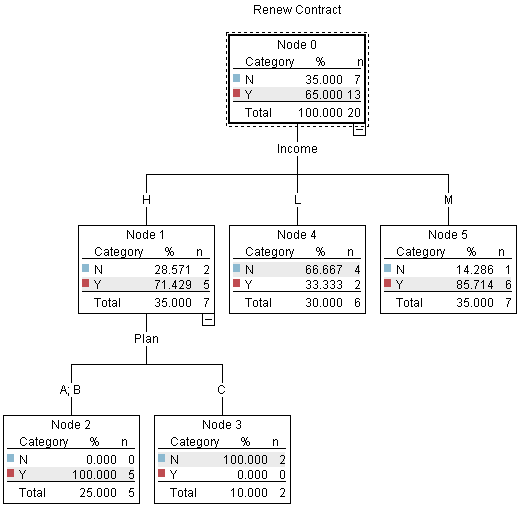
\includegraphics[width=.9\textwidth]{fig/default_tree.png}
\caption{Decision tree by C5.0 with default settings.}
\label{fig:default_tree}
\end{center}
\end{figure}

Decrease the level of pruning, a taller tree can be obtained shown in Figure~\ref{fig:new_tree}.

\begin{figure}[!ht]
\begin{center}
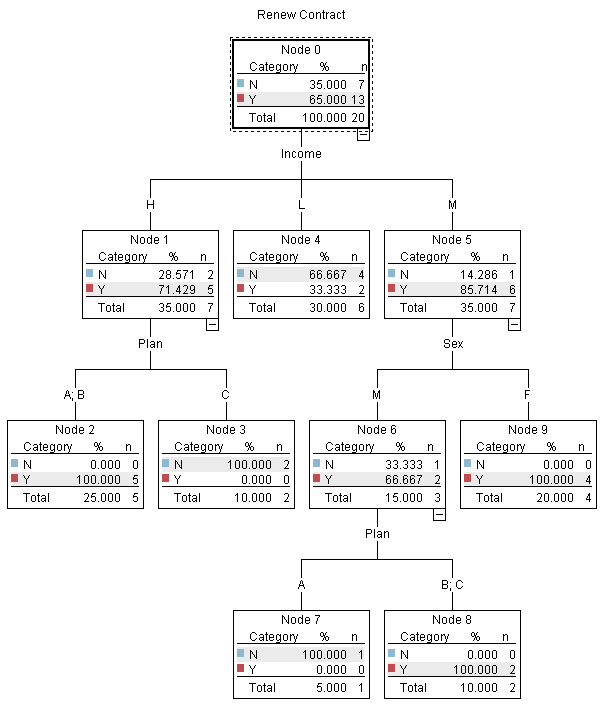
\includegraphics[width=\textwidth]{fig/new_tree.png}
\caption{Decision tree by C5.0 with less pruning.}
\label{fig:new_tree}
\end{center}
\end{figure}

Middle income group are extended to a more detailed sub-tree. However the new decision tree's error rate is 15\%, exactly the same as the much clearer default one. Both of them have 17 correct and 3 wrong using the 20-entry input as testing dataset. So I decided to keep the simpler one as the result from C5.0 in PASW.

The PASW generated tree is simper than manual calculated tree in that:
\begin{itemize}
\item Only 2 inputs, income and plan are used. Sex is not.
\item Low and middle income group are assigned a decision without further investigation on plan.
\end{itemize}

The reason for the simplicity is that C5.0 pruned some subtree if they do not offer sufficient information gain. Adding one more layer has both cost and gain. While the confidence of the decision rise, the amount of calculation increases, more time is necessary to generate/use the tree and more storage is used. C5.0, with its parameters, tries to find some balanced point between minimum cost and maximum accuracy(confidence).

\subsection{d}
Using the Na{\"\i}ve Bayesian approach, we calculate the probabilities of Yes or No decisions given other data of a customer. The calculation is:

$X_1 =  F S N M B$\\
$P(X_1|Yes) × P(Yes) = 8/13 × 4/13 × 4/13 × 6/13 × 5/13 × 13/20 = 0.0067224537$\\
$P(X_1|No) × P(No) = 4/7 × 2/7 × 4/7 × 1/7 × 1/7 × 7/20 = 0.000666389$\\

$X_2 = F S Y H C$\\
$P(X_2|Yes) × P(Yes) =8/13 × 4/13 × 9/13 × 5/13 × 4/13 × 13/20 = 0.0100836805$\\
$P(X_2|No) × P(No) =4/7 × 2/7 × 3/7 × 2/7 × 3/7 × 7/20 = 0.0029987505$\\

$X_3 = M Y Y L C$\\
$P(X_3|Yes) × P(Yes) =1/13^5 × 13/20 × 5 × 5 × 9 × 2 × 4 = 0.0031511502$\\
$P(X_3|No) × P(No) =1/7^5 × 7/20 × 3 × 4 × 3 × 4 × 3 = 0.0089962516$\\

$X_4 = F M N M A$\\
$P(X_4|Yes) × P(Yes) =1/13^5 × 13/20 ×8 × 4 × 4 × 6 × 4 = 0.005377963$\\
$P(X_4|No) × P(No) =1/7^5 × 7/20 × 4 × 1 × 4 × 1 × 3 = 0.0009995835$\\

$X_5 = M Y Y H B$\\
$P(X_5|Yes) × P(Yes) =1/13^5 × 13/20 ×5 × 5 × 9 × 5 × 5 = 0.0098473443$\\
$P(X_5|No) × P(No) =1/7^5 × 7/20 × 3 × 4 × 3 × 2 × 1 = 0.0014993753$\\

Based on the results, the prediction is \{Yes, Yes, No, Yes, Yes\}. The fact is \{Yes, No, Yes, No, Yes\}. 40\% is correct.

\subsection{e}
From best to worst: C5.0, ID3, Na{\"\i}ve Bayesian. (For this particular case only.)

The decision tree in Figure~\ref{fig:default_tree} successfully predicted 3 of the 5 records in testing dataset. Predictions for the testing dataset records based decision tree in Figure~\ref{fig:tree-level3} has a 100\% success rate. But if I randomly chose the decision ``No'' for ``Low-C'' node, the rate would be 80\%. Anyway, the prediction confidence of the ID3 decision tree is higher. Na{\"\i}ve Bayesian Approach offered the lowest success rate of 40\%, even lower than coin tossing. So the battle is left for ID3 and C5.0.

The ID3 tree has 4 layer while the C5.0 tree has only 3. In terms of node numbers, ID3 tree has 15 while the C5.0 tree has only 6.

C5.0 provided 60~75\% confidence of the ID3 tree with only 40\% tree-size. If we have more data, the difference success rate of ID3 tree and C5.0 tree over test datasets is not likely to be widened. But the difference in tree-size may be enlarged further. From this point of view, it is a better choice.

\section{Problem 3}
\subsection{a}
As different columns in the dataset has different units, the raw data needs normalization when calculating distances. The Mahalanobis distance is used here, which is defined as:

\begin{equation}
d(\vec{x},\vec{y})=\sqrt{\Sigma_{i=1}^{N}{(x_{i}-y_{i})^{2}\over \sigma_{i}^{2}}}
\end{equation}

$\sigma_{i}^{2}$ is the variance of the $i^{th}$ item in the vector.

Calculate the Mahalanobis distance between the query customer and each customer in the dataset.

\begin{table}[!ht]
\footnotesize
\caption{Distance between the query customer and each customer in the dataset.}
\begin{center}
\begin{tabular}{|c|c|}
\hline
Customer No. & Distance\\
\hline
1 & 2.134669658\\
2 & 1.665761127\\
3 & 1.172980416\\
4 & 1.68601554\\
5 & 1.333520147\\
6 & 2.670374446\\
7 & 1.73604759\\
8 & 1.049905052\\
9 & 1.137881937\\
10 & 3.206476268\\
11 & 2.698401638\\
12 & 1.451218709\\
13 & 0.417450221\\
14 & 1.249588594\\
15 & 0.931040981\\
16 & 1.642174336\\
17 & 3.050099327\\
18 & 0.44710203\\
19 & 1.862743077\\
20 & 0.536595894\\
\hline
\end{tabular}
\end{center}
\label{tab:dist1}
\end{table}%

The closest 5 are 13, 18, 20, 15 and 8. Among them, 3 switched, 1 stayed and 1 undecided. So the prediction for the query customer would be \textbf{Switch}.

\subsection{b}
Again, calculate the distances, but only using the \textit{Average Monthly Payment} and \textit{Total Calling Time} data.

\begin{table}[!ht]
\footnotesize
\caption{Distance between the second query customer and each customer in the dataset.}
\begin{center}
\begin{tabular}{|c|c|}
\hline
Customer No. & Distance\\
\hline
1 & 2.130083504\\
2 & 0.752860181\\
3 & 0.719271814\\
4 & 1.887532998\\
5 & 0.890583985\\
6 & 2.684491284\\
7 & 1.380705473\\
8 & 0.842978267\\
9 & 1.264445205\\
10 & 2.501359779\\
11 &1.553729197\\
12 &1.160523697\\
13 & 0.257991635\\
14 & 0.986859974\\
15 & 0.656593446\\
16 & 1.295358106\\
17 & 2.278424828\\
18 & 0.213756276\\
19 & 1.967165133\\
20 & 0.426519426\\
\hline
\end{tabular}
\end{center}
\label{tab:dist2}
\end{table}%

The closest 5 are 18, 13, 20, 15 and 3. To better predict the average duration of calls, we take the distance into consideration to weigh different references. Assume we have N closest points, the weight of the i'th point is calculated as:

\begin{equation}
w_{i} = {1/d_{i}^{2}\over \Sigma_{j=1}^{N}{1/d_{j}^{2}}}
\end{equation}

Then calculate the estimation of average call duration as:

\begin{equation}
t = \Sigma_{i=1}^{N}{w_{i}*t_{i}} = 7.29
\end{equation}

Therefore the average duration of calls of the query customer is estimated to be 7.29.

\subsection{c}
The value of $k$ is decided after the distance calculations. Starting from a small $k$, check if the prediction is possible and stable. If so, use that value; if not, increase $k$.

For the first question in this problem, the procedure of deciding the value of $k$ may be:
\begin{enumerate}
\item Starting with $k=2$, 1 stay and 1 undecided. Impossible to predict.
\item $k=3$, 1 stay, 1 undecided and 1 switch. Impossible to predict.
\item $k=4$, 1 stay, 1 undecided and 2 switches. Possible to predict, stability unknown.
\item $k=5$, 1 stay, 1 undecided and 3 switches. The prediction does not change, meaning it's stable to some extent. Stop.
\end{enumerate}

Different problems or different dataset distributions may lead to different criteria of stability. It is OK to check more, but the later data points are checked, the larger their distances are and thus the less they should contribute to the prediction.

For the second question, the 4th and 5th points are farther and their weight in prediction is so low that they actually can be dropped from the prediction. The weight distribution of the 5 points is \{0.469054826, 0.321995726, 0.117810426, 0.049712805, 0.041426217\}. The first 3 points add up to 91\% of the weight. If we set $k=3$, the prediction will be 7.26, which could be more accurate since the prediction is based on closer data points.

\section{Problem 4}
\subsection{a} % (fold)
\label{sub:4a}
Without pre-processing the data, only merging the two tables and then generating a decision tree with C5.0 in PASW, I was able to get two different results with different settings.

One tree I once got is a two-level tree with just one test on the symptoms column. It is so straightforward that it groups all the 0s, 1s, 2s and 3s and then the prediction goes like:
\begin{itemize}
	\item if the symptom is one of A, B, C, ..., M, then 0;
	\item if the symptom is one of N, O, ..., S, then 1;
	\item if the symptom is one of T, U, ..., W, then 2;
	\item otherwise, 3.
\end{itemize}
where A, B, C ... are sets of symptoms.

This tree is 100\% correct but is useless in that:
\begin{itemize}
	\item it ignores all the data except symptoms;
	\item even for symptoms, it does not support combinations that does not exist in the training dataset;
	\item the number of branches in the first level of the decision tree is virtually the number of different patterns of symptom descriptions in the training set, which is too large.
\end{itemize}

However useless the tree is, it does convey the message that \textbf{symptoms carry more information than other columns}. That is why the model ignores all other inputs but the symptoms.

To get rid of the mess in the symptoms column, I decided to exclude that column in the model to test if other columns can give a clearer tree. What I got is a single-node tree predicting the degree of thrombosis to be 0. In this way, PASW offered a model that is 84.34\% correct.

That means without processing the data, the modeler cannot grab much information from the current representation form of the inputs. And those branches those columns form are pruned due to low information gain.
% subsection a (end)

\subsection{b} % (fold)
\label{sub:4b}
In my data processing, the following discretization approaches are applied:
\begin{itemize}
	\item Derived flags whether P, S or D  appears in the ANA Pattern column. The distribution of that column shows that these 3 are the most frequent ones. Even though there is some orphan records that is 100\% confident to have a degree of 1, the only occurrence makes it less applicable to become a rule.
	\item Symptom reclassified to None, Thrombo~(any symptom with a prefix throm-), CNS(any combination that is related to CNS) and Other. In this way, the variety of symptoms is discretized into 4 bins.
	\item Diagnosis, similar to ANA Pattern, is converted to flags indicating whether there is a APS, SLE or MCTD in the record. These three are the most frequent ones in the distribution.
	\item Age by Examination is discretized into 3 bins, <33, 33 and >33. That is because 33 alone counts for around 50\% of the records after all the balancing in previous data processing.
\end{itemize}

To illustrate the effect of discretization, I summarized the quality of decision tree obtained after each approach listed above in Table \ref{tbl:accuracy}.

\begin{table}[!ht]
\caption{\label{tbl:accuracy} Effect of Data Processing Approaches}
\begin{center}
\begin{tabular}{|l|r|r|}
\hline
        \textbf{Approach} & \textbf{Accuracy \%} & \textbf{Tree size (nodes)}\\
\hline
                 Raw data &             84.34 &                          1\\
\hline
             Sex balanced &             85.66 &                          1\\
\hline
      ANA Pattern flagged &             85.66 &                          1\\
\hline
ANA Pattern flag balanced &             92.62 &                         13\\
\hline
 Symptom reclassification &             99.47 &                          7\\
\hline
         Symptom balanced &             99.86 &                         15\\
\hline
        Diagnosis flagged &               100 &                         23\\
\hline
Age by Examination binned &               100 &                         16\\
\hline
\end{tabular}
\end{center}
\end{table}

The major differences are:
\begin{itemize}
	\item After manual discretization, data in some columns are better utilized by the modeler. The most significant improvement comes from the reclassification of symptoms. This confirms the previous finding that the symptom column carries the most information.
	\item Processing the diagnosis column does improve the accuracy a little bit.
	\item Processing the ANA Pattern column does not make a difference. That means even after the processing, the column still carry little information and branches derived from those information are all pruned.
	\item Introducing a new discretization may increase the tree size since more tests are made to utilize the additional data.
	\item A new discretization may also decrease the tree size in that some branches with low information gain is replaced with new ones with higher information gain tapped from additional data.
\end{itemize}

Among all the trees I obtained, I would say the 99.47\% correct, 7-node tree, shown in Figure \ref{fig:tree_symptom_reclassified} and \ref{fig:accu_symptom_reclassified}, is the optimal one. Simple and accurate. In case accuracy is of much greater importance over speed, the last tree, shown in Figure \ref{fig:tree_age_3bin} and \ref{fig:accu_age_3bin} with 16 nodes, which is 100\% correct is also a good one to use.

\begin{figure}[!ht]
\begin{center}
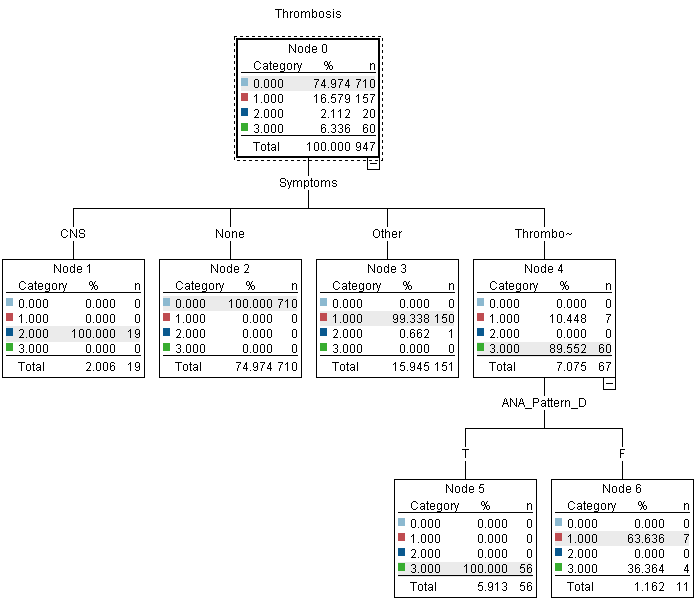
\includegraphics[width=\textwidth]{fig/tree_symptom_reclassified.png}
\caption{7-node tree obtained after reclassification of symptoms.}
\label{fig:tree_symptom_reclassified}
\end{center}
\end{figure}

\begin{figure}[!hb]
\begin{center}
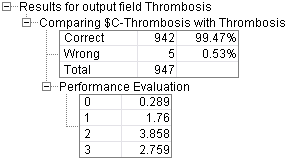
\includegraphics[scale=1]{fig/accu_symptom_reclassified.png}
\caption{Accuracy of the 7-node tree.}
\label{fig:accu_symptom_reclassified}
\end{center}
\end{figure}

\begin{figure}[!ht]
\begin{center}
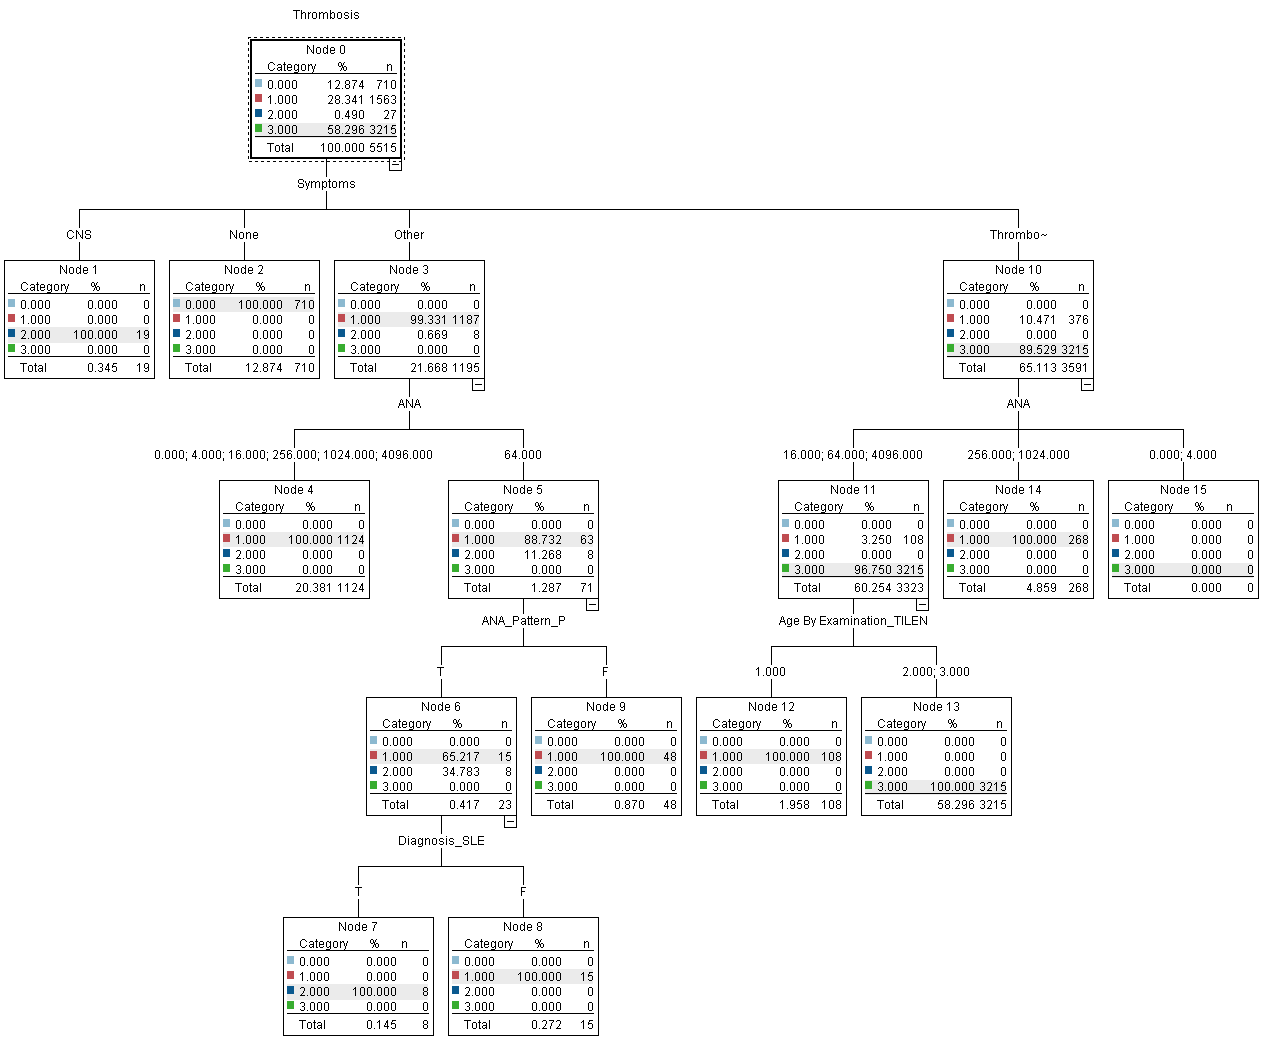
\includegraphics[width=\textwidth]{fig/tree_age_3bin.png}
\caption{16-node tree obtained after binning the age by examination into 3 groups.}
\label{fig:tree_age_3bin}
\end{center}
\end{figure}

\begin{figure}[!hb]
\begin{center}
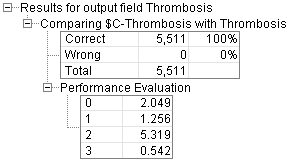
\includegraphics[scale=1]{fig/accu_age_3bin.png}
\caption{Accuracy of the 16-node tree.}
\label{fig:accu_age_3bin}
\end{center}
\end{figure}

When deriving all the new data columns, I converted all the input to lowercase before finding for flags. This is to eliminate the affect of different cases in the raw data.

There are also typos in the data. That does not affect my discretization as I only look for data that I am interested in and I have checked the data audit result. No typo will make a difference in my binning or reclassification.

The strategy is that I do not correct the data before I know for sure that column is used in the model. Then I try to avoid fixing each error by processing the data in a way that missing values/typos/illegal characters does not make a difference. The goal is to get an accurate model, the simpler the procedure is the better.
% subsection b (end)

\subsection{c} % (fold)
\label{sub:4c}
When I discretize the data, I follow these rules:
\begin{enumerate}
	\item I do not want to many bins. Acceptable numbers of bins are 2 (for True or False), 3 (for Young/Mid/Old), or 4 (for data like symptom with 3 frequent groups and many empty values).
	\item When the data can be easily grouped, group it.
	\item When group is not applicable or does not make sense (like grouping two unrelated diagnoses or symptoms), I try to use flags to break down the column into several flags. This is useful when only some of the data in that column actually contributes to the prediction. Just pick it out as a derived column.
\end{enumerate}

Varying the number of intervals for discretization does affect the decision tree generated.

When I first discretize the symptoms column, I reclassified the data into 3 bins instead of 4. CNS is not separated but marked "Others". The accuracy was 98.2 rather than 99.47 of the 4-bin approach. Though it is still a better tree than without the reclassification, it is not as good as it can be.

When discretize the age by examination, I tried 2, 3 and 4 bins. The principle is to make the number of records in each bin roughly the same.
As shown in Table \ref{tbl:accuracy}, the accuracy before binning the age has already reached 100\% without utilization of the age information. Additional information should not make the prediction less accurate, but it may simplify the tree by replacing some branches with more new ones with more information gain.

The result is that with 2 bins, the decision tree has 18 nodes. With 4 bins, the number is 23. Both are inferior to the 16-node tree with 3 bins.
Simplicity can be obtained with more rational discretization.
% subsection 4c (end)

\subsection{d} % (fold)
\label{sub:4d}
Other than discretization, I also derived age by examination from the original examination date and birthday information. I guess age does make a difference when predicting health status. The value is the year of examination date minus the year of birthday. I did not minus the year of "Today" since the age of patients now is not as relevant to their health state on the examination date.

The model does utilize the age data and the result is a simpler tree with same accuracy. The accuracy cannot be improved further since it is already 100\% before adding the age information.

Another important approach in my data processing is the generation of balanced nodes. When the distribution of different values is too uneven, it may lead to poor results. Check the "Data Audit" output and generate balanced nodes for those most uneven distributed data columns does help to get a more accurate decision tree.

In this case, balancing the ANA Pattern flags increased the accuracy from 85.66\% to 92.62\%. Actually it makes the tree so different that those flags derived are not pruned any more.
% subsection 4d (end)

The final modeling process is illustrated in Figure \ref{fig:stream1} and Figure \ref{fig:stream2}.
\begin{figure}[!ht]
\begin{center}
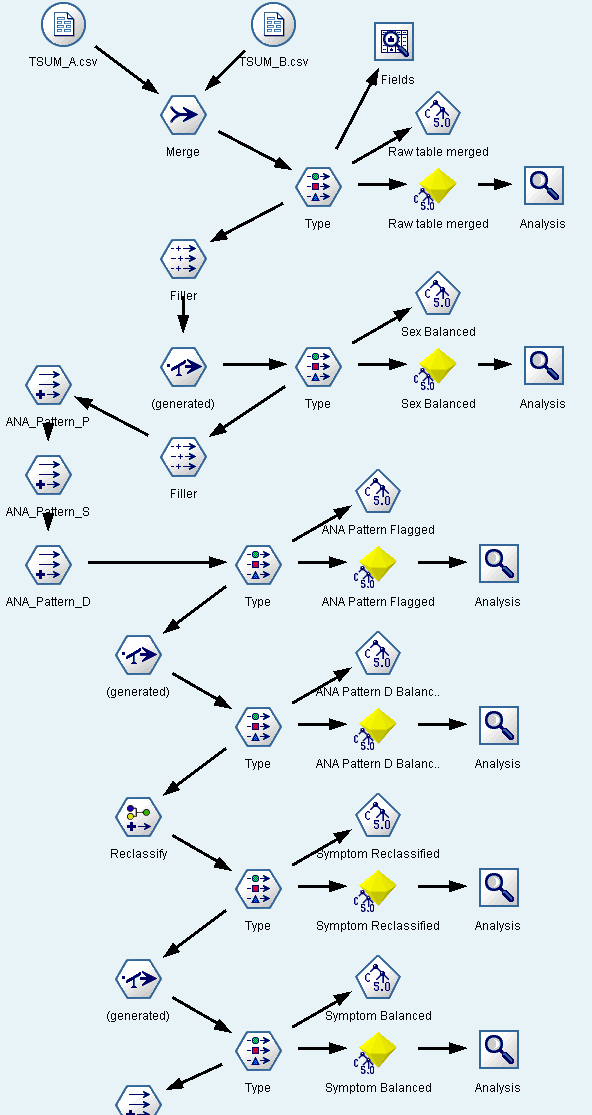
\includegraphics[width=.7\textwidth]{fig/pasw_stream_1.png}
\caption{The final PASW stream to obtain all the models.}
\label{fig:stream1}
\end{center}
\end{figure}

\begin{figure}[!ht]
\begin{center}
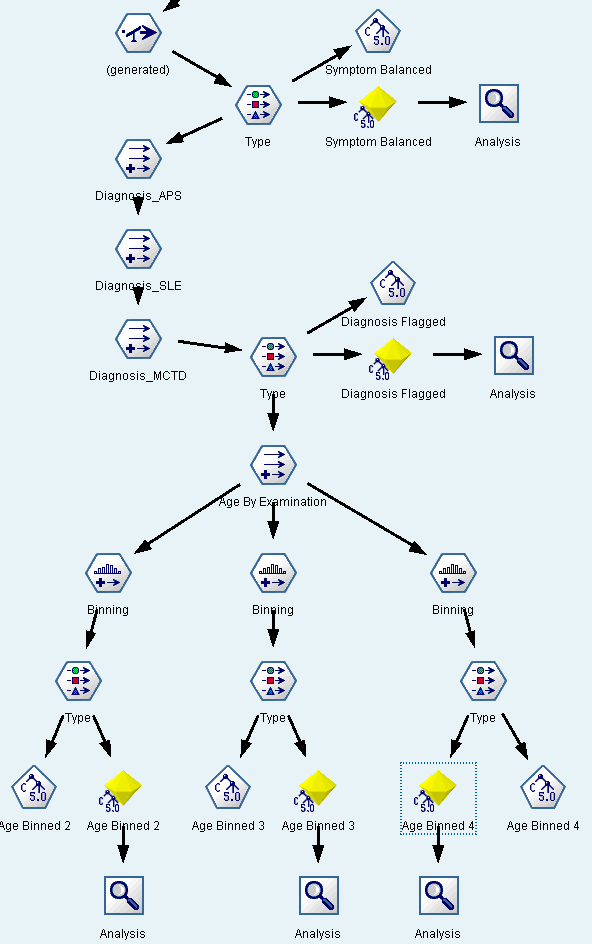
\includegraphics[width=.7\textwidth]{fig/pasw_stream_2.png}
\caption{Continued: The final PASW stream to obtain all the models.}
\label{fig:stream2}
\end{center}
\end{figure}

\end{document}  